\documentclass{beamer}
\usetheme{Boadilla}
%typical packages
\usepackage{tikz,amsfonts,amsmath,pgfplots}
\setcounter{MaxMatrixCols}{20}

\addtobeamertemplate{navigation symbols}{}{%
    \usebeamerfont{footline}%
    \usebeamercolor[fg]{footline}%
    \hspace{1em}%
    \insertframenumber/\inserttotalframenumber
}

%typical tikz stuff
\tikzstyle{vertex}=[circle, draw, inner sep=0pt, minimum size=6pt,fill=white]
\newcommand{\vertex}{\node[vertex]}
\usepackage{pgf}
\usetikzlibrary{arrows}
\pagestyle{empty}
\definecolor{zzttqq}{rgb}{0.6,0.2,0}
\definecolor{uququq}{rgb}{0.25,0.25,0.25}
\definecolor{xdxdff}{rgb}{0.49,0.49,1}
\definecolor{qqqqff}{rgb}{0,0,1}
\newcommand{\RR}{\mathbb{R}}


\title{Flows in Optimization}
\author{Stefano Fochesatto}
\institute{University of Alaska Fairbanks}
\date{\today}

\begin{document}
 \begin{frame}
\titlepage
\end{frame}




\begin{frame}
	\frametitle{Overview}
	\begin{center}
		\begin{itemize}
			\item Brief Introduction to Linear Optimization
			\vfill
			\item Geometry of Linear Programming
			\vfill
			\item Minimum Cost Network Flow Problem
			\vfill
			\item Different Flavors of Flow Problems
			\begin{itemize}
				\item Max Flow
				\item Min Cut 
				\item Shortest Path
				\item Assignment (Weighted Matching)
			\end{itemize}
			\vfill
			\item Lazy Snapping (Image Segmentation)
		\end{itemize}
	\end{center}
\end{frame}






\begin{frame}
	\frametitle{Linear Optimization}
	A \emph{Linear Programming(LP) Problem} is an optimization problem with a linear \emph{objective function} and linear \emph{constraints}. 
	A \emph{feasible set} $S$, is the set of points satisfying the constraints.
	\begin{figure}
		\caption{Example of an $LP$ Problem, and feasible set $S$.}
	\begin{columns}
		\begin{column}{.5\textwidth}
			\begin{center}
				\begin{align*}
					\mathop{\text{minimize: }}_{x}  z = -x_1  - &2x_2\\
				  \text{subject to: } -x_1 + x_2 &\leq 2\\
				  x_1 + x_2 &\leq 3\\
				  x_1, x_2 &\geq 0
				\end{align*}
				
			\end{center}
		\end{column}
		\begin{column}{.5\textwidth}
		\begin{center}
				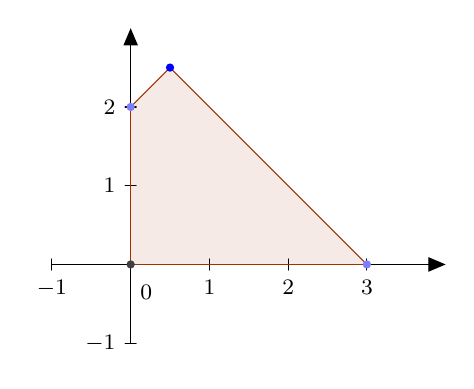
\begin{tikzpicture}[line cap=round,line join=round,>=triangle 45,x=1.0cm,y=1.0cm]
					\draw[->,color=black] (-1,0) -- (4,0);
					\foreach \x in {-1,1,2,3}
					\draw[shift={(\x,0)},color=black] (0pt,2pt) -- (0pt,-2pt) node[below] {\footnotesize $\x$};
					\draw[->,color=black] (0,-1) -- (0,3);
					\foreach \y in {-1,1,2}
					\draw[shift={(0,\y)},color=black] (2pt,0pt) -- (-2pt,0pt) node[left] {\footnotesize $\y$};
					\draw[color=black] (0pt,-10pt) node[right] {\footnotesize $0$};
					\clip(-1,-1) rectangle (4,3);
					\fill[color=zzttqq,fill=zzttqq,fill opacity=0.1] (0,2) -- (0.5,2.5) -- (3,0) -- (0,0) -- cycle;
					\draw [color=zzttqq] (0,2)-- (0.5,2.5);
					\draw [color=zzttqq] (0.5,2.5)-- (3,0);
					\draw [color=zzttqq] (3,0)-- (0,0);
					\draw [color=zzttqq] (0,0)-- (0,2);
					\begin{scriptsize}
						\fill [color=qqqqff] (0.5,2.5) circle (1.5pt);
					\fill [color=xdxdff] (3,0) circle (1.5pt);
					\fill [color=uququq] (0,0) circle (1.5pt);
					\fill [color=xdxdff] (0,2) circle (1.5pt);
					\end{scriptsize}
					\end{tikzpicture}
				\end{center}
			\end{column}
		\end{columns}
	\end{figure}
\end{frame}



\begin{frame}
	\frametitle{Linear Optimization}
	\begin{itemize}
		\item $LP$-Problems have \emph{convex (set)} feasible sets.
		\begin{figure}
			\caption {$S$ is a convex set.}
			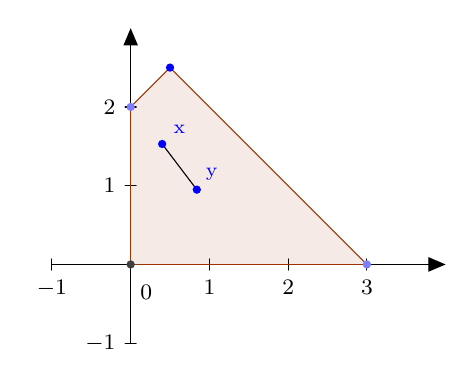
\begin{tikzpicture}[line cap=round,line join=round,>=triangle 45,x=1.0cm,y=1.0cm]
				\draw[->,color=black] (-1,0) -- (4,0);
				\foreach \x in {-1,1,2,3}
				\draw[shift={(\x,0)},color=black] (0pt,2pt) -- (0pt,-2pt) node[below] {\footnotesize $\x$};
				\draw[->,color=black] (0,-1) -- (0,3);
				\foreach \y in {-1,1,2}
				\draw[shift={(0,\y)},color=black] (2pt,0pt) -- (-2pt,0pt) node[left] {\footnotesize $\y$};
				\draw[color=black] (0pt,-10pt) node[right] {\footnotesize $0$};
				\clip(-1,-1) rectangle (4,3);
				\fill[color=zzttqq,fill=zzttqq,fill opacity=0.1] (0,2) -- (0.5,2.5) -- (3,0) -- (0,0) -- cycle;
				\draw [color=zzttqq] (0,2)-- (0.5,2.5);
				\draw [color=zzttqq] (0.5,2.5)-- (3,0);
				\draw [color=zzttqq] (3,0)-- (0,0);
				\draw [color=zzttqq] (0,0)-- (0,2);
				\draw (0.4,1.53)-- (0.84,0.95);
				\begin{scriptsize}
				\fill [color=qqqqff] (0.5,2.5) circle (1.5pt);
				\fill [color=xdxdff] (3,0) circle (1.5pt);
				\fill [color=uququq] (0,0) circle (1.5pt);
				\fill [color=xdxdff] (0,2) circle (1.5pt);
				\fill [color=qqqqff] (0.4,1.53) circle (1.5pt);
				\draw[color=qqqqff] (0.62,1.72) node {x};
				\fill [color=qqqqff] (0.84,0.95) circle (1.5pt);
				\draw[color=qqqqff] (1.03,1.14) node {y};
				\end{scriptsize}
				\end{tikzpicture}
		\end{figure}
		\begin{equation*}
			\alpha x + (1 - \alpha)y \in S \qquad \text{for all $0 \leq \alpha \leq 1$}
		\end{equation*}
		\item $LP$-Problems have \emph{convex (function)} objective functions.
		\begin{equation*}
			f(\alpha x + (1 - \alpha)y) \geq \alpha f(x) + (1 - \alpha)f(y) \qquad \text{for all $0 \leq \alpha \leq 1$}
		\end{equation*}
	\end{itemize}
\end{frame}



\begin{frame}
	\frametitle{Linear Optimization}
	\begin{itemize}
		\item An $LP$-problem is in \emph{standard form} if it is written in the following form where $b \geq 0$,
		\begin{align*}
			\mathop{\text{minimize: }}_{x}  z &= c^Tx\\
			\text{subject to: }Ax &= b\\
			x \geq 0
		\end{align*}  
		Note $x, c \in \RR^n$, $b \in \RR^m$. We call $A$ the \emph{constraint matrix}.

		\item All $LP$-problems can be written in standard form. 
	\end{itemize}
	\end{frame}



	\begin{frame}
		\frametitle{Linear Optimization}
		\begin{itemize}
			\item For an $LP$-problem in standard form, we define it's \emph{dual} $LP$-problem as, 
			\begin{figure}
				\caption{Primal and Dual $LP$-problems}
				\begin{columns}
					\begin{column}{.5\textwidth}
						\begin{center}
							\begin{align*}
								\mathop{\text{minimize: }}_{x}  z &= c^Tx\\
								\text{subject to: }Ax &= b\\
								x \geq 0
							\end{align*}  
						\end{center}
					\end{column}
					\begin{column}{.5\textwidth}
						\begin{center}
							\begin{align*}
								\mathop{\text{maximize: }}_{y}  w &= b^Ty\\
								\text{subject to: }A^Ty &= c\\
								y\geq 0
							\end{align*} 
						\end{center}
					\end{column}
				\end{columns}
			\end{figure}
		\end{itemize}
		\begin{block}{\emph{Strong Duality}}
		 For a pair of Primal-Dual $LP$-problems if one has an optimal solution then so does the other, and the optimal objective values are equal.
		\end{block}
	\end{frame}


	\begin{frame}
		\frametitle{Linear Optimization}
		\begin{itemize}
			\item We say a solution is $x$ is a \emph{basic feasible solution} if,
			\begin{itemize}
				\item The columns of $A$ corresponding to $x_i \neq 0$ are linearly independent.
				\item $x \geq 0$ and $Ax = b$. 
  			\end{itemize} 
			\vfill
						  \item For any $LP$-problem, if $S$ is bounded and non-empty then by convexity there exist a finite optimal solution and such a solution is a basic feasible solution.
						  \vfill
			  \begin{block}{\emph{Fundamental Theorem of Linear Programming}}
				  For an $LP$-problem in standard form, $x$ is an extreme point of $S$ if and only if $x$ is a basic feasible solution.
			  \end{block}
		\end{itemize}
	\end{frame}




	\begin{frame}
		\frametitle{Geometry of Linear Programming}
		To summarize\dots
		\begin{itemize}
			\item Every $LP$-problem can be written in standard form. 
			\item For a standard form $LP$-problem, the optimal solution is an extreme point of the feasible set $S$.
			\item Strong Duality allows us to certify that our solution is the optimal one. 
		\end{itemize}
		The \emph{Simplex Algorithm}, which is actually used to solve $LP$-problems, is based on these principles. 
	\end{frame}

	\begin{frame}
		\begin{center}
			That's great\dots but what's the point?
		\end{center}
	\end{frame}

	\begin{frame}
		\begin{center}
			Flow Problems $\subset$ $LP$-Problems \footnotemark 
		\end{center}

	\footnotetext[1]{At least, the ones we've seen}
	\end{frame}

	\begin{frame}
		\frametitle{Preface on Terminology}
		The field of Optimization is very opinionated about terminology (just like Graph Theory)
		\begin{itemize}
			\item \emph{Network} == \emph{Graph}
			\item \emph{flow} is also an arbitrary unit assigned to each vertex. (ex: the vertex $s$ has a flow of $f(s, N(s))$)
			\item Edges are also assigned a \emph{cost}, which is the cost of moving one unit of flow across said edge. 
		\end{itemize}

	\end{frame}

	\begin{frame}
		\frametitle{Minimum Cost Network Flow Problem}
		\begin{itemize}
			\item Suppose we have a directed graph $G = (V, E)$, let $b$ be a vector of flows assigned to each vertex, and $c$ be a vector of costs for each arc. 
			\vfill
			\item Vertex $i$ with $b_i > 0$ is a \emph{source}, $b_i < 0$ is a \emph{sink}.  
			\item We define \emph{Supply} $S$, and \emph{Demand} $D$ as,  
			\begin{equation*}
					S = \sum_{\{i :b_i > 0\}}b_i, \qquad D = \sum_{\{i: b_i < 0\}}b_i.
			\end{equation*}
			\item It is necessary that $S - D = 0$, such a network is called \emph{balanced}.  
		\end{itemize}
		\begin{figure}
			\begin{center}
			  \caption{Graph $G = (V, E)$ with flow $b$ and weights $c$}
			  \includegraphics[width=.90\textwidth]{SampleNetwork.png}
			\end{center}
		  \end{figure}
	\end{frame}

	\begin{frame}
		\frametitle{Minimum Cost Network Flow Problem}
		A solution to the such a problem, is a flow $f$ which satisfies the supply and demand ($|f| = S = -D$) but minimizes cost. 
		\begin{itemize}
			\item Objective Function ($x$ is a flow):
			\begin{equation*}
				\mathop{\text{minimize: }}_{x}  z = c^Tx
			\end{equation*}
			where $x_{(i, j)} \in x$ represents flow through arc $(i, j)$, and $c_{(i, j)} \in c$ is cost through arc $(i, j)$. 
			\vfill
			\item Constraints:
			\begin{equation*}
				\sum_{j}x_{i, j} - \sum_{k}x_{k, i} = b_i \text{ for all $i \in V$}. 
			\end{equation*}
			This ensures $x$ satisfies supply and demand, for example,
				\begin{equation*}
					x_{1, 2} + x_{1,3} = 50,
					\qquad x_{2, 4} + x_{2, 6} - x_{1, 2} = 0.
				  \end{equation*}
			\item Key Observation: $x$ represents edges, $b$ represents vertices....
		\end{itemize}
	\end{frame}

	\begin{frame}
		\frametitle{Minimum Cost Network Flow Problem}
		\begin{itemize}
			\item Observe that the following is the constraint matrix $A$, for the problem above. 
			\begin{equation*}
				A = 
				\begin{bmatrix}
					1 & 1  &    &    &    &    &    &    &    &    &   \\
					-1 &    & 1  & 1  &    &    &    &    &    &    &  \\
					& -1 &    &    & 1  & 1  &    &    &    &    &  \\
					&    & -1 &    & -1 &    & 1  & 1  &    &    &  \\
					&    &    &    &    & -1 & -1 &    & 1  & 1  &  \\
					&    &    & -1 &    &    &    & -1 & -1 &    & 1\\
					&    &    &    &    &    &    &    &    & -1 & -1\\
				\end{bmatrix}
			\end{equation*}
			\item Minimum and maximum (capacity) flow through arc $x_{(i, j)}$, denoted by vectors $L$ and $U$ are enforced by inequality constraints. 
			\item Described as an $LP$-problem, 
			\begin{align*}
				\mathop{\text{minimize: }}_{x}  z &= c^Tx\\
			  \text{subject to: }Ax &= b\\
			  L \leq&x\leq U
			\end{align*}
		\end{itemize}
	\end{frame}


	\begin{frame}
		\frametitle{Maximum Flow}
		\begin{itemize}
			\item Suppose we have a directed graph $G = (V, E)$, capacities $u_{(i, j)}$, a source vertex 1, and sink vertex $m$ and we wish to find the maximum flow $f$.
			\item Represented as an optimization problem,
			\begin{align*}
				\mathop{\text{maximize: }}_{x, f} &z = f\\
				\text{subject to: } &\sum_{j}x_{1, j} - \sum_{k}x_{k, 1} = f,\\
				&\sum_{j}x_{i, j} - \sum_{k}x_{k, i} = 0, \quad i = 2, \dots, m - 1\\
				&\sum_{j}x_{m, j} - \sum_{k}x_{k, m} = -f,\\
				&0 \leq x_{i, j} \leq u_{i, j}.
			\end{align*} 
			\item explain...
		\end{itemize}
		\end{frame}
			
		\begin{frame}
			\frametitle{Maximum Flow}
			\begin{itemize}
			\item Add arc $(m, 1)$ with $u_{(m, 1)} = \infty$ to uncouple, we get
			\begin{align*}
				\mathop{\text{minimize: }}_{x} &z = -x_{m, 1}\\
				\text{subject to: } &\sum_{j}x_{i, j} - \sum_{k}x_{k, i} = 0, \quad i = 1, \dots, m\\
				&0 \leq x_{i, j} \leq u_{i, j}
			\end{align*}
			\vfill
			\item This is a Minimum Cost Network Flow problem in disguise 
			\begin{itemize}
				\item Let $b = 0$, $c_{(m,1)} = -1$ and zero otherwise, $U = u$ and $L = 0$.
				
				\item All of costs were zero \dots 
			\end{itemize}
		\end{itemize}
	\end{frame}



	\begin{frame}
		\frametitle{Minimum Cut}
		\begin{itemize}
			\item We have shown in class that the Maximum Flow = Minimum Cut,
			\begin{itemize}
				\item Strong Duality implies that the Dual $LP$-problem computes the minimum cut. 
			\end{itemize} 
			\item Represented as an optimization problem (Dual of original Max-flow), 
			\begin{align*}
				\mathop{\text{minimize: }}_{y, v}  &w = \sum u_{i, j} v_{i, j}\\
				\text{subject to: } y_m - y_1 &= 1\\
				y_i - y_j &+ v_{i, j} \geq 0, \quad \text{for all arcs $(i, j)$}\\
				v_{i, j} &\geq 0
			\end{align*}
			\item $y$ represents indicator for disjoint sets $N_1$ and $N_0$, $v$ represents the indicator for the separating set of arcs. 
		\end{itemize}
	\end{frame}


	\begin{frame}
		\frametitle{Shortest Path}
		\begin{itemize}
			\item Finding the shortest path between two vertices $v_0$ and $v_f$, on a directed graph $G = (V, E)$. 
			\begin{itemize}
				\item Minimum Cost Network Flow problem with one source $v_0$ and one sink $v_f$ and flows are 1 and -1 respectively. 
				\item $c_{(i, j)}$ is distance. 
			\end{itemize}
			\vfill
			\item More efficient algorithms exists, the more popular ones require $c_{(i, j)} \geq 0$. 
		\end{itemize}
	\end{frame}


	\begin{frame}
		\frametitle{Assignment (Weighted Matching)}
		\begin{itemize}
			\item Recall the stable matching problem (medical students to residencies).
			\begin{itemize}
				\item Let $c_{i, j}$ be 'happiness' score for matching student $i$ with program $j$. 
				\item We want to find a matching which maximizes happiness.  
			\end{itemize}
			\item Let $G = (A \cup B, E)$ be a directed complete bipartite graph
			\item $A$ represents student, $B$ represents programs, arcs go from $A$ to $B$
			\item Vertices in $A$ are all sources with flow 1, with $B$ defined analogously. 
			\item Cost are defined by $c_{i, j}$ and instead we maximize the objective function. 
			\vfill
		\end{itemize}		
	\end{frame}



	\begin{frame}
		\frametitle{Lazy Snapping}
		\begin{itemize}
			\item Image segmentation, is the process by which a subject and background are identified. 
			\begin{figure}
				\caption{Example Segmentation}
				\begin{center}
					\includegraphics[width = .65\textwidth]{segmentation.png}
				\end{center}
				\end{figure}
				\vfill
			\item Lazy Snapping is a technique for image segmentation which uses flows.
			\begin{itemize}
				\item User selects some source and sink pixels.
				\item The image is converted into a min-cut flow problem. (this part is hard)
				\item Resulting disjoint sets identify the subject and background.  
			\end{itemize} 
			\end{itemize}
	\end{frame}

	\begin{frame}
		\frametitle{Lazy Snapping}
		\begin{itemize}
			\item It's relatively easy to frame this as an optimization problem.
			\item We define an energy function, $E(X)$ where $X$ is indicator for subject pixels. 
			\begin{equation*}
				E(X) = \sum_{i \in V} E_1(x_i) + \lambda \sum_{(i, j) \in E} E_2(x_i, x_j). 
			\end{equation*}
			\item $E_1$ and $E_2$ are defined in Li et al.(2004)
			\begin{itemize}
				\item $\sum_{i \in V} E_1(x_i)$ is small when pixels identified by $X$ are the same color. 
				\item $E_2(x_i, x_j)$ identifies pixels $x_i, x_j$ where $X(x_i) \neq X(x_j)$, and is large when the pair of pixels are a similar color.  
			\end{itemize}
			\item Converting energy functions like $E$ into flow problems is described in Boykov \& Jolly (2001).  
		\end{itemize}
	\end{frame}


	\begin{frame}
		\frametitle{Lazy Snapping}
		\begin{figure}
			\caption{Image to Flow}
			\begin{center}
				\includegraphics[width = .6\textwidth]{image2flow.png}
			\end{center}
			\end{figure}
	\end{frame}

	\begin{frame}
		\frametitle{Lazy Snapping}
		\begin{itemize}
			\item Demo Time !!!
		\end{itemize}
	\end{frame}



%%%%%%END%%%%%%%
\end{document}
